\clearpage
\section{Guia prático: o que aparece nos quantis de cada score?}
\label{app:quantiles}

\subsection{Antes de ordenar: duas perguntas diferentes}
Imagine uma ação que pode aumentar a conversão. Para cada perfil de cliente, conhecemos a probabilidade de converter sem a ação, $\mu_0(x)=\mu(a_0,x)$, e com a ação, $\mu_1(x)=\mu(a,x)$. Aqui, ``com ação'' significa aplicar a mesma alternativa $a$ a todos; ``sem ação'' significa aplicar a mesma referência $a_0$. Os exemplos são inteiramente fictícios, com probabilidades conhecidas. Não há modelos ajustados, outcomes sorteados ou erro de estimação.

Dois scores respondem a perguntas úteis, mas diferentes:
\begin{align*}
S_{\mathrm{CATE}}(x)&=\mu_1(x)-\mu_0(x)
&&\text{(quanto aumenta a chance de converter?)},\\
S_{\mathrm{lift}}(x)&=\frac{\mu_1(x)}{\mu_0(x)}-1
&&\text{(quanto aumenta em relação à chance inicial?)}.
\end{align*}
\textbf{CATE é um ganho absoluto; lift é um ganho proporcional.} Neste apêndice, CATE sempre designa a diferença aditiva. O score relativo também pode ser expresso como razão $R=1+\mathrm{lift}$ ou log-razão $g=\log(1+\mathrm{lift})$: ambos produzem o mesmo ranking do lift, pois são transformações estritamente crescentes.

\noindent\textbf{Unidades, sem ambiguidade.} Passar de 2\% para 3,6\% significa ganhar \emph{1,6 ponto percentual}, ou 0,016 na escala de probabilidade. O lift é $3{,}6/2-1=80\%$. Em 1\,000 pessoas iguais a esse perfil, isso corresponde a passar de 20 para 36 conversões esperadas: \emph{16 conversões adicionais}. São expectativas contrafactuais, não a identificação de quais 16 pessoas mudariam de decisão.

\begin{table}[H]
\centering\small
\caption{Cinco perfis fictícios, cada um com 20\% da população. O contraste de tratamento é o mesmo em todas as linhas.}
\label{tab:quantile_profiles}
\begin{tabular}{lrrrrr}
\toprule
Perfil & Pessoas & Base (\%) & Com ação (\%) & CATE (p.p.) & Lift (\%) \\
\midrule
A & 1000 & 2,00 & 3,60 & 1,60 & 80,00 \\
B & 1000 & 4,00 & 6,00 & 2,00 & 50,00 \\
C & 1000 & 8,00 & 10,40 & 2,40 & 30,00 \\
D & 1000 & 16,00 & 19,20 & 3,20 & 20,00 \\
E & 1000 & 25,00 & 28,75 & 3,75 & 15,00 \\
\bottomrule
\end{tabular}

\end{table}

\textbf{A e E deixam a diferença clara.} O perfil A ganha 80\% sobre uma base de 2\%: seu CATE é 1,6 p.p. O perfil E ganha 15\% sobre uma base de 25\%: seu CATE é 3,75 p.p. Portanto, A tem o maior lift e E tem o maior ganho absoluto. Isso decorre da identidade
\[
\underbrace{\mathrm{CATE}(x)}_{\text{ganho absoluto}}
=\underbrace{\mu_0(x)}_{\text{conversão-base}}
\times\underbrace{\mathrm{lift}(x)}_{\text{ganho relativo}}.
\]
Um método DML pode aprender um alvo aditivo ou relativo, dependendo da equação usada. ``DML'' descreve a construção de estimação e não determina a unidade do score. No pacote deste projeto, os Q-Learners e os DMLs entregam respostas relativas; o CATE aditivo exige também uma estimativa de $\mu_0(x)$, multiplicada pelo lift.

\clearpage
\subsection{Os mesmos clientes, duas ordenações e cinco grupos}
Ordenamos as 5\,000 pessoas do menor para o maior score e formamos cinco grupos de 1\,000: \textbf{Q1 tem os menores scores e Q5 os maiores}. Cada perfil tem um score distinto e ocupa exatamente um quintil; nenhum empate é dividido. Na tabela, ``extras'' significa $1\,000\times\mathrm{CATE}$, e lift do grupo significa razão das suas médias de conversão, menos um.

\begin{table}[H]
\centering\small
\setlength{\tabcolsep}{5pt}
\caption{O que se encontra em cada quintil. A população é a mesma; apenas a ordenação muda.}
\label{tab:quantile_rankings}
\begin{tabular}{lllrrrrr}
\toprule
Score & Quantil & Perfil & \shortstack{Base\\(\%)} & \shortstack{Com ação\\(\%)} & \shortstack{CATE\\(p.p.)} & \shortstack{Lift\\(\%)} & \shortstack{Extras por\\1\,000} \\
\midrule
CATE & Q1 & A & 2,00 & 3,60 & 1,60 & 80,00 & 16,0 \\
CATE & Q2 & B & 4,00 & 6,00 & 2,00 & 50,00 & 20,0 \\
CATE & Q3 & C & 8,00 & 10,40 & 2,40 & 30,00 & 24,0 \\
CATE & Q4 & D & 16,00 & 19,20 & 3,20 & 20,00 & 32,0 \\
CATE & Q5 & E & 25,00 & 28,75 & 3,75 & 15,00 & 37,5 \\
Lift & Q1 & E & 25,00 & 28,75 & 3,75 & 15,00 & 37,5 \\
Lift & Q2 & D & 16,00 & 19,20 & 3,20 & 20,00 & 32,0 \\
Lift & Q3 & C & 8,00 & 10,40 & 2,40 & 30,00 & 24,0 \\
Lift & Q4 & B & 4,00 & 6,00 & 2,00 & 50,00 & 20,0 \\
Lift & Q5 & A & 2,00 & 3,60 & 1,60 & 80,00 & 16,0 \\
\bottomrule
\end{tabular}

\end{table}

\begin{figure}[H]
\centering
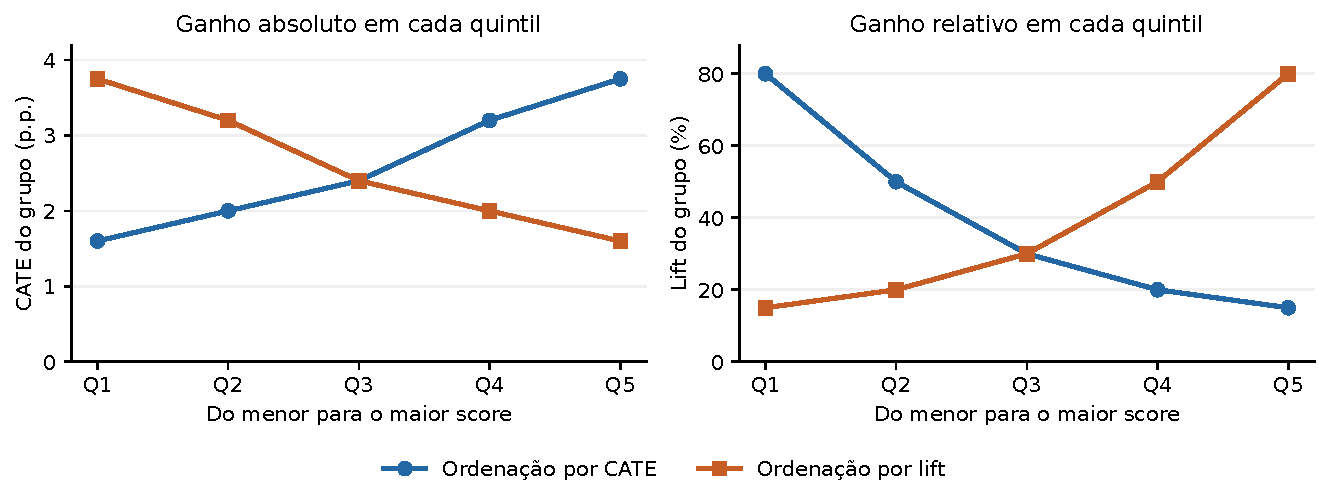
\includegraphics[width=\linewidth]{figures/quantile_cate_vs_lift.pdf}
\caption{Azul: grupos formados pelo score de CATE. Laranja: grupos formados pelo score de lift. Cada painel avalia ambos os rankings na mesma unidade. Q5 reúne pessoas diferentes nas duas curvas. Valores exatos da população sintética, sem incerteza amostral.}
\label{fig:quantile_rankings}
\end{figure}

\textbf{Como ler o gráfico.} O ranking azul cresce no painel de CATE, mas cai no de lift. O laranja faz o inverso. Um score pode ordenar perfeitamente o seu alvo e ter uma curva decrescente na outra escala. Isso não é falha de calibração: os alvos são diferentes.

\textbf{Se só houver capacidade para 1\,000 pessoas:} selecionar Q5 por CATE escolhe E e gera 37,5 conversões adicionais esperadas; selecionar Q5 por lift escolhe A e gera 16. Com custo e valor por conversão iguais, o primeiro maximiza conversões incrementais neste exemplo. O segundo seleciona a maior resposta proporcional. Lift alto, isoladamente, não significa maior lucro ou maior número de conversões extras.

\clearpage
\subsection{Quando o lift empata: o baseline pode ordenar o CATE}
Agora mantenha as mesmas conversões-base e imponha um lift de 20\% para todos. A conversão aumenta proporcionalmente da mesma forma em todos os perfis, enquanto o ganho em pontos percentuais aumenta com o baseline.

\begin{table}[H]
\centering\small
\caption{Resposta relativa constante: todos têm o mesmo lift.}
\label{tab:quantile_constant}
\begin{tabular}{lrrrr}
\toprule
Perfil & Base (\%) & Com ação (\%) & CATE (p.p.) & Lift (\%) \\
\midrule
A & 2,00 & 2,40 & 0,40 & 20,00 \\
B & 4,00 & 4,80 & 0,80 & 20,00 \\
C & 8,00 & 9,60 & 1,60 & 20,00 \\
D & 16,00 & 19,20 & 3,20 & 20,00 \\
E & 25,00 & 30,00 & 5,00 & 20,00 \\
\bottomrule
\end{tabular}

\end{table}

O score de CATE ordena A, B, C, D e E; seus quintis coincidem com a ordem do baseline. O score de lift vale 20\% para todas as pessoas: \textbf{não existem cinco faixas distintas de resposta relativa}. Um software pode desempatar por posição da linha ou aleatoriamente, mas esses grupos não representam diferenças de lift. Por isso, não fabricamos uma curva de quintis relativos neste caso. Se um modelo estimado produzir pequenas diferenças, a ordenação pode refletir apenas ruído e precisa de validação fora da amostra.

\subsection{A média dos lifts individuais pode não ser o lift do grupo}
Para um grupo $G$, as quantidades usadas na tabela e no gráfico são
\[
\mathrm{CATE}_G=\E[\mu_1(X)\mid G]-\E[\mu_0(X)\mid G],\qquad
\mathrm{lift}_G=\frac{\E[\mu_1(X)\mid G]}{\E[\mu_0(X)\mid G]}-1.
\]
A média dos CATEs individuais é o CATE do grupo. A média simples dos lifts individuais, em geral, não é o lift do grupo. Veja dois perfis de mesmo tamanho:

\begin{table}[H]
\centering\small
\caption{Dois perfis com pesos iguais: média individual de 55\%, lift do grupo de 18,18\%.}
\label{tab:quantile_mixture}
\begin{tabular}{lrrrr}
\toprule
Perfil & Base (\%) & Com ação (\%) & CATE (p.p.) & Lift (\%) \\
\midrule
U & 1,00 & 2,00 & 1,00 & 100,00 \\
V & 10,00 & 11,00 & 1,00 & 10,00 \\
Grupo (médias) & 5,50 & 6,50 & 1,00 & 18,18 \\
\bottomrule
\end{tabular}

\end{table}

A média dos lifts é $(100\%+10\%)/2=55\%$. Porém, a conversão média passa de 5,5\% para 6,5\%, de modo que o lift do grupo é $6{,}5/5{,}5-1=18{,}18\%$. A fórmula correta é
\[
\mathrm{lift}_G
=\frac{\E[\mu_0(X)\,\mathrm{lift}(X)\mid G]}{\E[\mu_0(X)\mid G]}:
\]
os pesos são proporcionais às conversões-base esperadas. A média simples de 55\% é outro resumo legítimo, desde que seja rotulada como \emph{média dos lifts individuais}. No exemplo principal, cada quintil contém um único perfil, então os dois resumos coincidem dentro do quintil. Na população inteira, o CATE é 2,59 p.p. e o lift do grupo é 23,55\%, independentemente do ranking escolhido.

\clearpage
\subsection{O mesmo raciocínio vale para tratamento contínuo}
Em um tratamento discreto, podemos comparar braço 1 com braço 0. Em um tratamento contínuo, precisamos fixar duas doses e a direção da mudança: por exemplo, $a_0=0$ e $a=1$ em uma escala normalizada. Uma curva que reproduz exatamente os cinco perfis da Tabela~\ref{tab:quantile_profiles} é
\[
\mu(t,x)=b(x)\exp\{t\log(1+\ell(x))\},\qquad 0\leq t\leq1,
\]
com $b(x)$ igual ao baseline e $\ell(x)$ igual ao lift daquela tabela. Em $t=0$, a conversão é $b(x)$; em $t=1$, é $b(x)(1+\ell(x))$. Todas as probabilidades permanecem entre zero e um. Para o contraste $0\to1$, os CATEs, lifts e rankings são os mesmos do exemplo discreto.

Para outra mudança $a_0\to a$, o score relativo nessa curva passa a ser
\[
\mathrm{lift}(a,a_0;x)=\exp\{(a-a_0)\log(1+\ell(x))\}-1,
\]
e o score absoluto é $\mu(a_0,x)\times\mathrm{lift}(a,a_0;x)$. \textbf{A comparação precisa usar o mesmo contraste nos dois scores.} Uma derivada $s(t,x)=\partial_t\log\mu(t,x)$ mede variação log-relativa por unidade de dose; ela não é o lift de uma mudança finita. Nesta curva, $s=\log(1+\ell)$, e o lift requer aplicar a exponencial ao produto da inclinação pela mudança de dose. Se a curva tiver curvatura, usa-se a diferença de log-respostas entre as duas doses, ou a integral de $s$, e não apenas uma derivada local.

\subsection{Como fazer a avaliação com scores aprendidos}
Os exemplos anteriores ensinam a ler o alvo, não demonstram a qualidade preditiva de um estimador. Com dados observados, um protocolo simples é:
\begin{enumerate}
\item \textbf{Definir a comparação antes de avaliar.} Fixar população, outcome, janela temporal, doses ou braços e escala do tratamento. Construir um score para CATE e outro para lift para esse mesmo contraste.
\item \textbf{Separar treino de avaliação.} Treinar os modelos em uma amostra e congelar suas previsões antes de usar os outcomes de teste. Formar os quintis a partir dessas previsões, sem consultar os outcomes. Registrar os cortes e o tratamento dos empates; para comparação, usar a mesma população de teste nos dois rankings.
\item \textbf{Estimar as duas conversões em cada grupo.} Em um experimento binário com probabilidades de alocação constantes, médias por braço são uma referência; com alocação variável, usar os pesos do desenho. Em dados observacionais discretos, usar médias ajustadas, por exemplo sinais AIPW com nuisances fora da amostra e overlap adequado. Para dose contínua, usar o estimador de dose-resposta ou de intervenção estocástica apropriado: não basta aplicar a fórmula AIPW binária a doses exatas.
\item \textbf{Mostrar as duas escalas e sua incerteza.} A partir das médias estimadas, calcular diferença em p.p. e razão menos um. Reportar tamanho do grupo, conversão-base, suporte e intervalos compatíveis com o desenho. Uma curva monotônica de previsões por construção não valida o efeito; a evidência vem da avaliação independente dos grupos.
\end{enumerate}
Comparar apenas a conversão observada de Q5 com a de Q1 mistura baseline, composição dos grupos e alocação de tratamento. Isso não identifica CATE nem lift causal. Em dados sintéticos podemos calcular as duas médias contrafactuais exatas; em dados reais é necessário estimá-las sob as hipóteses de identificação.

\noindent\textbf{Reprodução.} Executar \texttt{quantile\_examples.py} recria as tabelas, CSVs e o gráfico. O script verifica as identidades de agregação, a inversão do perfil selecionado em Q5, o empate de lift constante e o contraexemplo da média dos lifts.
